\subsection{Sprint-3} \label{sec:sprint-3}
Il terzo sprint (figura \ref{fig:backlog-sprint-3}) ha segnato il completamento delle funzionalità del
gioco principale e ha posto le basi per l'integrazione dei minigiochi. le funzionalità aggiunte sono state:
\begin{itemize}
    \item tiro di dadi iniziale per decidere il primo giocatore
    \item movimento intelligente del nemico
    \item rigenerazione del tabellone di gioco
    \item doppio tiro di dado per il vincitore di un minigioco
\end{itemize}
\begin{figure}[ht!]
    \centering
    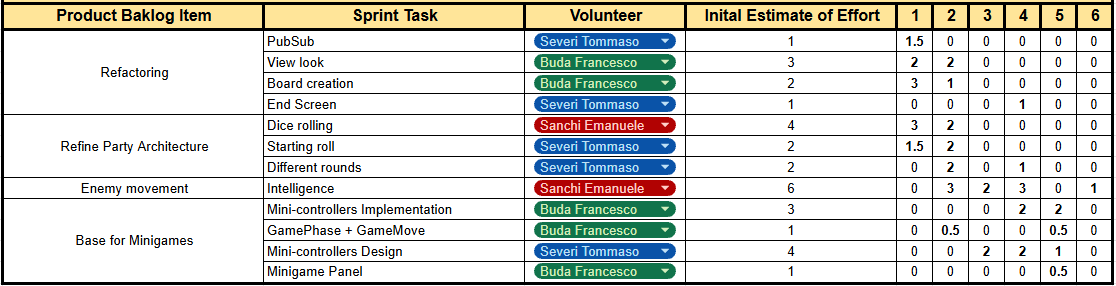
\includegraphics[width=1\textwidth]{figures/backlog-sprint-3.png}
    \caption{Backlog per lo Sprint-3}
    \label{fig:backlog-sprint-3}
\end{figure}